% 
% ---------------------------------------------------------------
% Copyright (C) 2012-2018 Gang Li
% ---------------------------------------------------------------
%
% This work is the default powerdot-tuliplab style test file and may be
% distributed and/or modified under the conditions of the LaTeX Project Public
% License, either version 1.3 of this license or (at your option) any later
% version. The latest version of this license is in
% http://www.latex-project.org/lppl.txt and version 1.3 or later is part of all
% distributions of LaTeX version 2003/12/01 or later.
%
% This work has the LPPL maintenance status "maintained".
%
% This Current Maintainer of this work is Gang Li.
%
%

\documentclass[
 size=12pt,
 paper=smartboard, %a4paper, smartboard, screen
 mode=present, %present, handout, print
 display=slides, % slidesnotes, notes, slides
% nohandoutpagebreaks,
% pauseslide,
style=tuliplab,
% nopagebreaks,clock
% hlentries=true,
% hlsections = true,
pauseslide,
fleqn,leqno]{powerdot}

\hypersetup{pdfpagemode=FullScreen}
% \usepackage[toc,highlight,blackslide,slidesonly,sounds,HA]{HA-prosper}

\usepackage{amssymb}
\usepackage{amsmath} 
\usepackage{rotating}
\usepackage{graphicx}
\usepackage{boxedminipage}
\usepackage{media9}
\usepackage{rotate}
\usepackage{calc}
\usepackage[absolute]{textpos}
\usepackage{psfrag,overpic}
\usepackage{fouriernc}
\usepackage{pstricks,pst-node,pst-text,pst-3d,pst-grad}
\usepackage{moreverb,epsfig,color,subfigure}
\usepackage{color}
\usepackage{pstricks}
\usepackage{pstricks-add}
\usepackage{pst-text}
\usepackage{pst-node, pst-tree}
\usepackage{booktabs}
\usepackage{etex}
\usepackage{breqn}
\usepackage{multirow}
\usepackage{gitinfo2}

\usepackage{listings}
\lstset{frameround=fttt, 
frame=trBL, 
stringstyle=\ttfamily,
backgroundcolor=\color{yellow!20},
basicstyle=\footnotesize\ttfamily}
\lstnewenvironment{code}{
\lstset{frame=single,escapeinside=`',
backgroundcolor=\color{yellow!20},
basicstyle=\footnotesize\ttfamily}
}{}


\usepackage{fouriernc}
\usepackage{hyperref}

%%%%%%%%%%%%%%%%%%%%%%%%%%%%%%%%%%%%%%%%%%%%%%%%%%%%%%%%%%%%%%%%%%%%%%%%
% title
% TODO: Customize to your Own Title, Name, Address
%
\title{FLIP01 MIDTERM PRESENTATION}
\author{Zebin Ju
Xi'an Shiyou University 
% \href{mailto:gangli@acm.org}{gangli@acm.org}
% \and % more authors
}
\date{\today}


% Customize the setting of slides
\pdsetup{
% theslide=\arabic{slide}~/~\pageref*{lastslide},
% theslide=\arabic{slide},
rf=\href{http://www.tulip.org.au}{
Last Changed by: \textsc{\gitCommitterName}\ \gitVtagn-\gitAbbrevHash\ (\gitAuthorDate)
},
cf={FLIP01 MIDTERM PRESENTATION},
%trans=Fade,
%list={labelsep=1em,leftmargin=*,itemsep=0pt,topsep=5pt,parsep=0pt},
% counters={theorem,lemma},
% randomdots,dmaxdots=80
}


\begin{document}

\maketitle 
\begin{slide}[toc=,bm=]{Overview}
  \tableofcontents[content=sections]
\end{slide}

  \section{Problem Description}

  \begin{slide}{Definition}
  %\tableofcontents[content=currentsection,type=1]
  Rotten tomato movie review data set is a movie review corpus for emotional analysis. It is an opportunity for us to build your idea of Emotional Analysis on rotten tomato data set. It is required to mark phrases with five levels of values: negative, some negative, neutral, some positive, positive. Negative sentences, satire, conciseness, language ambiguity and other obstacles make this task very challenging.
  %\begin{slide}{The overview of the question }
    %\vspace{2cm}
    %\setlength{\parindent}{1.5em}
    %You are given 5 years of store-item sales data, and asked to predict 3 months of sales for 50 different items at 10 different stores.
  %\end{slide}
  %\begin{slide}{Data Set}
  %\begin{itemize}
   % \item datalist
   % \begin{description}
    %  \item [date]\,  Date of the sale
     % \item [store] Store ID
     % \item [item]\,  Item ID
     % \item [sales] Number of items sold at a particular store on a particular date.
   % \end{description}
    \

  %\item Display the data set 
 % \begin{table}[htbp]  \centering
   % \caption{The head of the data set}
   % \label{tbl:data information}
   % \begin{tabular}{ccccccc}
    % \hline
      % after \\: \hline or \cline{col1-col2} \cline{col3-col4} ...
    %  & date & store & item & sales\\
     % \hline
     % 0 & 2013-01-01 & 1 & 1 & 13 \\
     % 1 & 2013-01-02 & 1 & 1 & 11 \\
     % 2 & 2013-01-03 & 1 & 1 & 14 \\
     % 3 & 2013-01-04 & 1 & 1 & 13 \\
    %  4 & 2013-01-05 & 1 & 1 & 10 \\
     % \hline 
      %\bottomrule
   % \end{tabular}
 % \end{table}
  %\end{itemize}
%\end{slide}
 % \begin{slide}[toc=,bm=]{Overview}
    %\tableofcontents[content=sections]
    %\end{slide}
    %\section{Second section}
   %\begin{slide}[toc=,bm=]{Main contents}
    %\tableofcontents[content=currentsection,type=1]
    %\end{slide}
    %\begin{slide}{Problem analysis by using data visualization}
      %\begin{itemize}
      %\item List the directories and files and load  data set
      %\item The introduction of the data set
      %\item Plot statistical charts and see the sale pattern
      %\item Variation in scale of the sale transacted
      %\item Store total sales
      %\item Item total sales
      %\item All store's performance
      %\item Individual pattern of store's and item's sales
      %\end{itemize}
    %\end{slide} 

\section{Problem Analysis}
%\begin{slide}{Data Analysis}
  %The dataset consists of tab delimited files and phrases in the rotten tomatoes dataset. Each phrase has a phraseid. Each sentence has a sentenceid.
%\vspace{1.5cm}
 %\begin{itemize}
 % \item Figures
%  \item 0 for negative
 %%% \item 1 for somewhat negative
  %\item 2 for neutral
 % \item 3 for somewhat positive
  %\item 4 for positive
  %\begin{itemize}
    %\item About sale pattern
    %\item About sales volume’s distribution
    %\item About total sales of all stores and items
    %\item About  performance
  %\end{itemize}
%\end{itemize}
%\end{slide}

\begin{slide}[toc=,bm=]{Type Of Review}
  Next, we can see the category distribution of comments. From the figure, we can see that emotion tag 2, that is, the most neutral comments. 
\begin{figure}[ht]%插入图片
  \centering%用于居中
  \includegraphics[scale=0.9]{D:/software/flip01/pictures/type of review.eps}
  \caption{Type of review}%图片标题
  \end{figure}
  \vspace{1cm}
 
\end{slide}
%\begin{slide}{Plot statistical charts and see the sale pattern} 
%By using the matplotlib to plot the photoes which describe the sale pattern
%\vspace{1cm}
%\begin{figure}[ht]%插入图片
  %\centering%用于居中
  %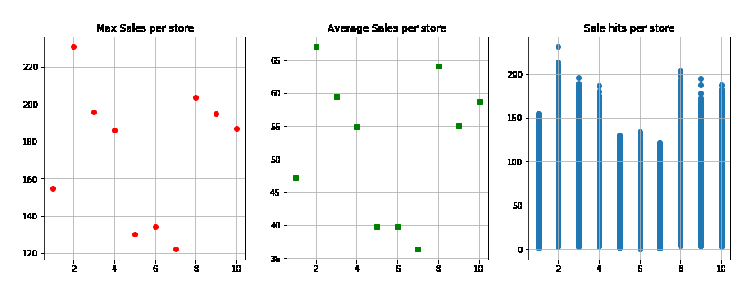
\includegraphics[scale=0.9]{E:/tulip-flip/templatex-master/powerdot-tuliplab/logos/0003.eps}
  %\caption{Displaying the sale pattern}%图片标题
  %\end{figure}
  %\vspace{0.5cm}
%From the figures we can know that 2nd store is the topper and 7th store is the least revenue generating one
%\end{slide}

%\begin{slide}[toc=,bm=]{visualization}
 % Displaying the distribution of sales volume
  %\begin{figure}[ht]%插入图片
  %  \centering%用于居中
    %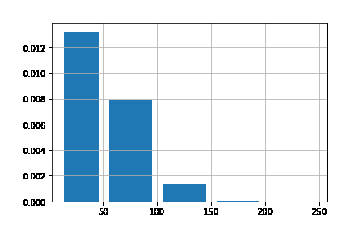
\includegraphics[scale=1.0]{E:/tulip-flip/templatex-master/powerdot-tuliplab/logos/0004.eps}
    %\caption{sales volume's distribution}%图片标题
    %\end{figure}
   % \vspace{1cm}
   % From this figure we can know that more and more sales volume is belong to [0,50].
  %\end{slide}

%\begin{slide}{Variation in scale of the sale transacted}
%Displaying the distribution of sales volume 
%\vspace{1cm}
%\begin{figure}[ht]%插入图片
  %\centering%用于居中
  %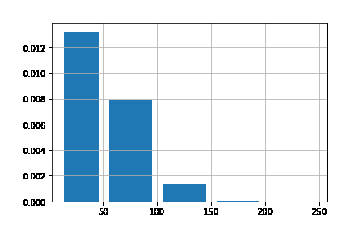
\includegraphics[scale=1.0]{E:/tulip-flip/templatex-master/powerdot-tuliplab/logos/0004.eps}
  %\caption{sales volume's distribution}%图片标题
  %\end{figure}
  %\vspace{1cm}
  %From this figure we can know that more and more sales volume is belong to [0,50]
%\end{slide}

%\begin{slide}[toc=,bm=]{visualization}
  %Displaying the total sales of the stores
  %\begin{figure}[ht]%插入图片
    %\centering%用于居中
   %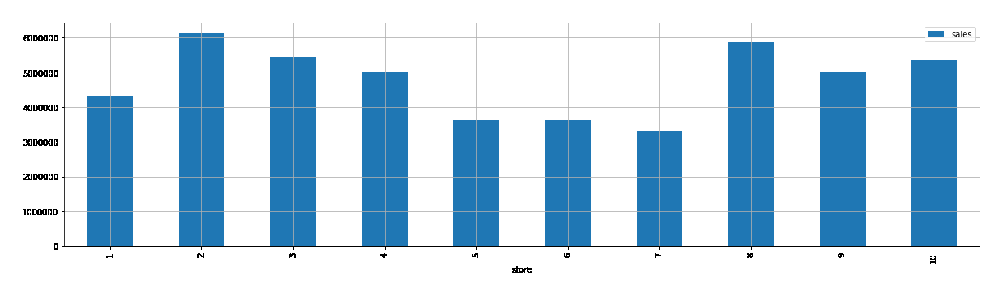
\includegraphics[scale=1.0]{E:/tulip-flip/templatex-master/powerdot-tuliplab/logos/0005.eps}
    %\caption{The total sales of all stores}%图片标题
   % \end{figure}
   % \vspace{0.5cm}
   %From this figure we can know that 2nd store is the topper of the all stores
  %\end{slide}

%\begin{slide}{Store total sales}
%Displaying the total sales of the stores 
%\vspace{1.0cm}
%\begin{figure}[ht]%插入图片
  %\centering%用于居中
  %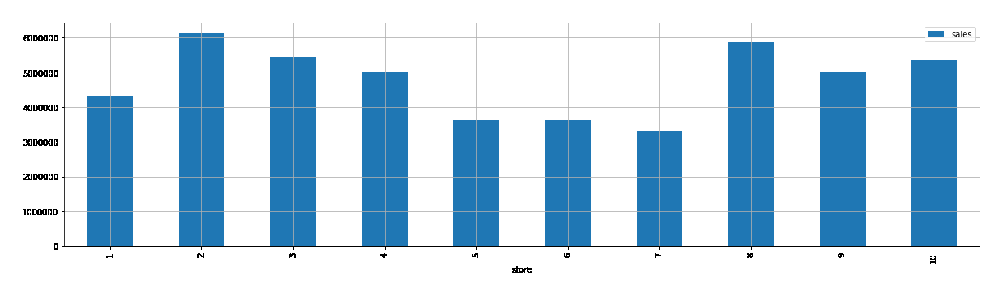
\includegraphics[scale=1.0]{E:/tulip-flip/templatex-master/powerdot-tuliplab/logos/0005.eps}
  %\caption{The total sales of all stores}%图片标题
  %\end{figure}
  %\vspace{0.5cm}
  %From this figure we can know that 2nd store is the topper of the all stores
%\end{slide}

%\begin{slide}[toc=,bm=]{visualization}
  %Displaying the total sales of the items
  %\vspace{0.8cm} 
  %\begin{figure}[ht]%插入图片
    %\centering%用于居中
    %\includegraphics[scale=0.7]{E:/tulip-flip/templatex-master/powerdot-tuliplab/logos/0006.eps}
    %\caption{The total sales of all items}%图片标题
    %\end{figure}
    %\vspace{0.3cm}
    %From this figure we can know the total sales of all items.Obviously,we can know every item's sales.
  %\end{slide}


%\begin{slide}{Item total sales}
  %Displaying the total sales of the items 
  %\vspace{0.8cm}
  %\begin{figure}[ht]%插入图片
    %\centering%用于居中
    %\includegraphics[scale=0.7]{E:/tulip-flip/templatex-master/powerdot-tuliplab/logos/0006.eps}
    %\caption{The total sales of all items}%图片标题
   % \end{figure}
    %\vspace{0.3cm}
   % From this figure we can know the total sales of all items.Obviously,we can know every item's sales
%\end{slide}

%\begin{slide}[toc=,bm=]{visualization}
  %Displaying the all store's performance over the time
  %\vspace{1cm} 
  %\begin{figure}[ht]%插入图片
    %\centering%用于居中
    %\includegraphics[scale=0.7]{E:/tulip-flip/templatex-master/powerdot-tuliplab/logos/0007.eps}
    %\caption{The performance of all stores}%图片标题
    %\end{figure}
    %From this figure we can know every stores sales changing overtime.
  %\end{slide}


%\begin{slide}{All store's performance}
%Displaying the all store's performance over the time
%\vspace{1cm}
%\begin{figure}[ht]%插入图片
  %\centering%用于居中
  %\includegraphics[scale=0.7]{E:/tulip-flip/templatex-master/powerdot-tuliplab/logos/0007.eps}
  %\caption{The performance of all stores}%图片标题
  %\end{figure}
  %From this figure we can know every stores sales changing overtime
%\end{slide}

%\begin{slide}[toc=,bm=]{visualization}
 % Displaying the all items' performance over the time
  %\vspace{1.2cm} 
 %\begin{figure}[ht]%插入图片
   % \centering%用于居中
   % \includegraphics[scale=0.7]{E:/tulip-flip/templatex-master/powerdot-tuliplab/logos/0008.eps}
   % \caption{The performance of all stores items}%图片标题
    %\end{figure}
   % From this figure we can know every item sales changing overtime .
  %\end{slide}


%\begin{slide}{All item's performance}
  %Displaying the all items' performance over the time
  %\vspace{1.2cm}
  %\begin{figure}[ht]%插入图片
    %\centering%用于居中
    %\includegraphics[scale=0.7]{E:/tulip-flip/templatex-master/powerdot-tuliplab/logos/0008.eps}
    %\caption{The performance of all stores items}%图片标题
    %\end{figure}
    %From this figure we can know every item sales changing overtime 
  %\end{slide}

  %\begin{slide}[toc=,bm=]{visualization}
   % Displaying the performance of the individual score and item
   %\vspace{1cm} 
   % \begin{figure}[ht]%插入图片
     % \centering%用于居中
      %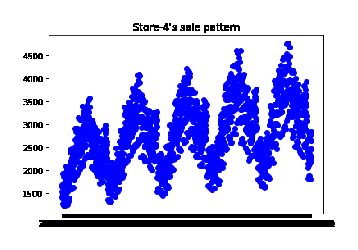
\includegraphics[scale=0.9]{E:/tulip-flip/templatex-master/powerdot-tuliplab/logos/0009.eps}
     % 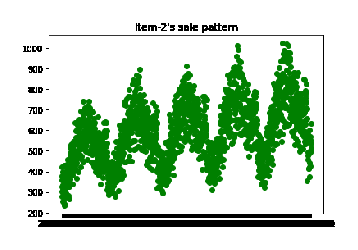
\includegraphics[scale=0.9]{E:/tulip-flip/templatex-master/powerdot-tuliplab/logos/0010.eps}
     % \caption{The performance of the individual store and item}%图片标题
     % \end{figure}
     % \vspace{0.5cm}
     % From this figure we can know individual pattern of item's sale and store's sale.
    %\end{slide}


%\begin{slide}{Individual pattern of store's and item's sale}
%Displaying the performance of the individual score and item
%\vspace{1cm}
%\begin{figure}[ht]%插入图片
  %\centering%用于居中
  %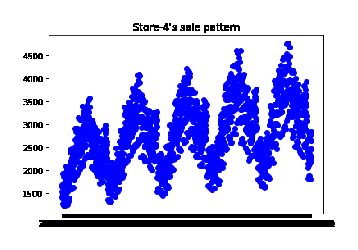
\includegraphics[scale=0.9]{E:/tulip-flip/templatex-master/powerdot-tuliplab/logos/0009.eps}
  %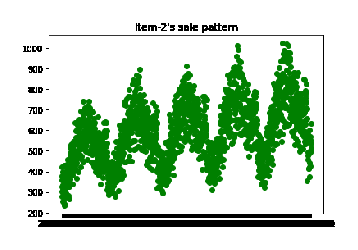
\includegraphics[scale=0.9]{E:/tulip-flip/templatex-master/powerdot-tuliplab/logos/0010.eps}
  %\caption{The performance of the individual store and item}%图片标题
  %\end{figure}
  %\vspace{0.8cm}
  %From this figure we can know individual pattern of item's sale and store's sale
%\end{slide}

%\begin{slide}{Data Preparation}
 % Through the data visualization before, we can intuitively recognize the changes in sales. However, to forecast sales for the 
 % next three months, we need to extract some new features. From the previous figure we can see that the sales are related to the
 % characteristics of the year, month, season, etc., so we can add some new features.

%\begin{itemize}
 % \item New features
  %\ 
  %\begin{description}
    %\item[dayofweek]- The day of the week. Monday is indicated by 0, Tuesday is indicated by 1, and so on.
    %\item[is_weekend]-  Determine if this day is a weekend. 
    %\item[day]- The day of the month.
    %\item[year]- Judging year. 
    %\item[dayofyear]- The day of the year.
    %\item[weekofyear] - The week of the year.
    %\item[sales_mean_lag_90]-Calculate 90 days from the day before, and then start from this day, the average of the first seven days.
    %\item[sales_std_lag_90]-  Calculate 90 days from the day, and then start from this day, the standard deviation of the first seven days. 
  %\end{description} 
%\end{itemize}
%\end{slide}

%\begin{slide}{Data Preparation}
  %\begin{table}[htbp]  \centering
   % \tiny
   %% \caption{New features presentation}
   % \label{tbl:1data information}
    %\begin{tabular}{cccccccccccccccc}
     %\hline
      % after \\: \hline or \cline{col1-col2} \cline{col3-col4} ...
     % & date & store & item & sales& dayofweek & is_weekend & day & month & year & dayofyear & weekofyear & sales_mean_lag_90 & sales_std_lag_90 \\
     % \hline
    % & 2017-12-22 & 10 & 50 & 75& 4& 0 & 22 & 12 & 2017 & 356 & 51 & 86.714286 & 15.882005 \\
    % & 2017-12-23 & 10 & 50 & 70& 5& 1 & 23 & 12 & 2017 & 357 & 51 & 85.571429 & 14.397420 \\
    % & 2017-12-24 & 10 & 50 & 76& 6& 1 & 24 & 12 & 2017 & 358 & 52 & 85.857143 & 13.837492 \\ 
    % & 2017-12-25 & 10 & 50 & 51& 0& 0 & 25 & 12 & 2017 & 359 & 52 & 85.142857 & 14.076323 \\
     %& 2017-12-26 & 10 & 50 & 41& 1& 0 & 26 & 12 & 2017 & 360 & 52 & 86.285714 & 13.123951 \\
     % & 2017-12-28 & 10 & 50 & 59& 3& 0 & 28 & 12 & 2017 & 362 & 52 & 84.285714 & 12.351981 \\ 
     %& 2017-12-29 & 10 & 50 & 74& 4& 0 & 29 & 12 & 2017 & 363 & 52 & 85.142857 & 13.533028 \\
     % & 2017-12-31 & 10 & 50 & 82& 6& 1 & 31 & 12 & 2017 & 365 & 52 & 86.285714 & 11.542881 \\
     % \hline 
      %\bottomrule
    %\end{tabular}
  %\end{table}
%\vspace{1cm}
%This is the tail of the data set which add the new features
%\end{slide}

\section{Text Feature Extraction}

\begin{slide}[toc=,bm=]{Text Feature Extraction}

  It is the process of transforming text data into feature vector. Machine learning algorithm often can't directly process text data, so it needs to transform text data into numerical data.
  \begin{itemize}
  \item CountVectorizer \ 

  %There are many machine learning methods for solving regression problems. This moment I will choose the lightGBM model
  \item TfidfVectorizer
 % \[SMAPE=\frac{100\%}{n}\sum_{t=1}^n\frac{|F_t-A_t|}{(|A_t|+|F_t|)/2} \]
\end{itemize}
\end{slide}

%\begin{slide}[toc=,bm=]{Forcasting}
% \item Do a model training
 % \item Model prediction
 % \item Model evaluation
  %\item Re-train model
  %\item Feature importance
 % \item test predations
%\end{itemize}
%\end{slide}

%\begin{slide}[toc=,bm=]{Forcasting}
 % \begin{figure}[ht]%插入图片
  %  \centering%用于居左
   % 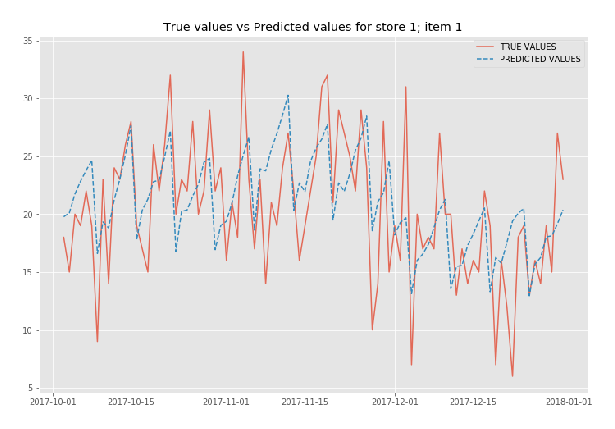
\includegraphics[scale=0.7]{E:/tulip-flip/templatex-master/powerdot-tuliplab/logos/012.eps}
    %\caption{The value vs predict}%图片标题
    %\end{figure}
%\vspace{1cm}
%Figure 8 is the first prediction based on the model.
%\end{slide}

%\begin{slide}[toc=,bm=]{Forcasting}
 % \begin{figure}[ht]%插入图片
    %\centering%用于居左
    %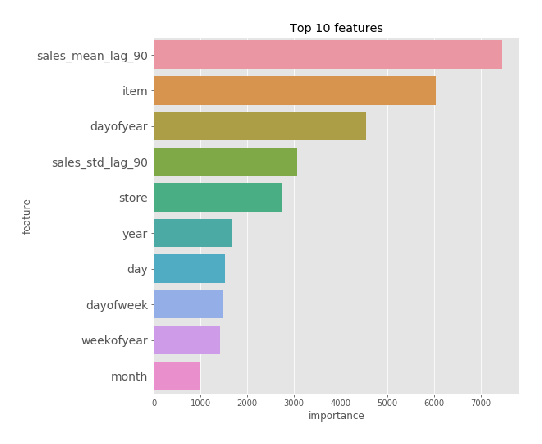
\includegraphics[scale=0.7]{E:/tulip-flip/templatex-master/powerdot-tuliplab/logos/013.eps}
    %\caption{Top 10 importabce features}%图片标题
   % \end{figure}
%\vspace{1cm}
%Figure 9 shows ten features with high feature importance.
%\end{slide}


%\begin{slide}[toc=,bm=]{Forcasting}
  %\begin{figure}[ht]%插入图片
    %\centering%用于居中
    %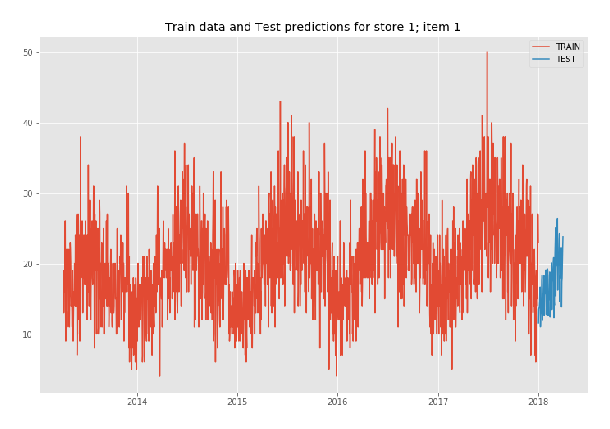
\includegraphics[scale=0.7]{E:/tulip-flip/templatex-master/powerdot-tuliplab/logos/014.eps}
    %\caption{The test prediction}%图片标题
   % \end{figure}
%\vspace{1cm}
%Figure 10 is a new prediction based on the model to get the results needed for this problem.
%\end{slide}

\section{Methods}
\begin{slide}[toc=,bm=]{Naive Bayes}
\begin{description}
  Naive Bayes is a classification algorithm based on probability theory, which can predict classification by considering feature probability.
  \item[CountVectorizer] 0.6715045495322312
  \item[TfidfVectorizer] 0.6308070613866461
  %\item[Modeling] Choose the suitable model parameters.
  %\item[Prospcting] I woule like to select multiple models for comparison later.
\end{description}
\begin{figure}[ht]%插入图片
  \centering%用于居中
  \includegraphics[scale=0.9]{D:/software/flip01/pictures/cv Naive Bayes.eps}
  \includegraphics[scale=0.9]{D:/software/flip01/pictures/tv Naive Bayes.eps}
  \caption{CountVectorizer and tfidfVectorizer}%图片标题
  \end{figure}
  \vspace{0.8cm}
\end{slide}

\section{Thanks for watching}


%\begin{slide}[toc=,bm=]{}
  %\tableofcontents[content=sections]
  %\end{slide}
  %\section{Third section}
  %\begin{slide}[toc=,bm=]{Acknowledge}
  %\tableofcontents[content=currentsection,type=1]
  %\end{slide}
%\begin{slide}{Acknowledge}
%\vspace{3.5cm}
%\centering
%\huge
%\textit{Thank you for watching the slides} 
%\end{slide}
\end{document}

\endinput
